\section{Conclusion and future developments}
\subsection{Possible future developments}
%  possibile introdure altri symmetry breaking
One of possible future development is to introduce new symmetry breaking as follows: once we have found a solution, we can represent it as a bi-dimensional matrix $M$, in which every value $M_{i,j} \in \{0,\dots,N\}$, then it is possible to encode each circuit as a sub-matrix of $M$, such that for a generic circuit $v$, $M_{x_{v} \dots w_v, y_v \dots h_v} = v$. A possible example, representing the solution of figure \ref{fig:future}, is the following:
\begin{center}
    $ \begin{bmatrix}
        1 & 1 & 1 & 3 & 3 & 3 & 3 & 3 \\
        1 & 1 & 1 & 3 & 3 & 3 & 3 & 3 \\
        1 & 1 & 1 & 3 & 3 & 3 & 3 & 3 \\
        4 & 4 & 4 & 4 & 4 & 2 & 2 & 2  \\
        4 & 4 & 4 & 4 & 4 & 2 & 2 & 2  \\
        4 & 4 & 4 & 4 & 4 & 2 & 2 & 2  \\
        4 & 4 & 4 & 4 & 4 & 2 & 2 & 2  \\
        4 & 4 & 4 & 4 & 4 & 2 & 2 & 2
    \end{bmatrix}  $
    \label{Solution as Matrix}
\end{center}

In order to reduce the number of symmetries to be computed by the solver we can impose an ordering between the matrix $M$ and other possible permutation of it. In particular we can state that:
\begin{itemize}
    \item to remove the original version flipped vertically:
        \begin{equation*}
            \text{lex\_lesseq}(\text{array1d(M)}, M[i, j] \text{ where } i \in \{HEIGHT,\dots,1\}, j \in \{1, \dots, WIDTH\});
        \end{equation*}
    \item to remove the rotated version by 180°:
        \begin{equation*}
            \text{lex\_lesseq}(\text{array1d(M)}, M[i, j] \text{ where } i \in \{HEIGHT,\dots,1\}, j \in \{WIDTH, \dots, 1\});
        \end{equation*}
    \item to remove the 180 degrees rotated and flipped vertically version:
        \begin{equation*}
            \text{lex\_lesseq}(\text{array1d(M)}, M[i, j] \text{ where } i \in \{1,\dots,HEIGHT\}, j \in \{WIDTH, \dots, 1\}).
        \end{equation*}
\end{itemize}

\begin{figure}[!h]
 \centering
 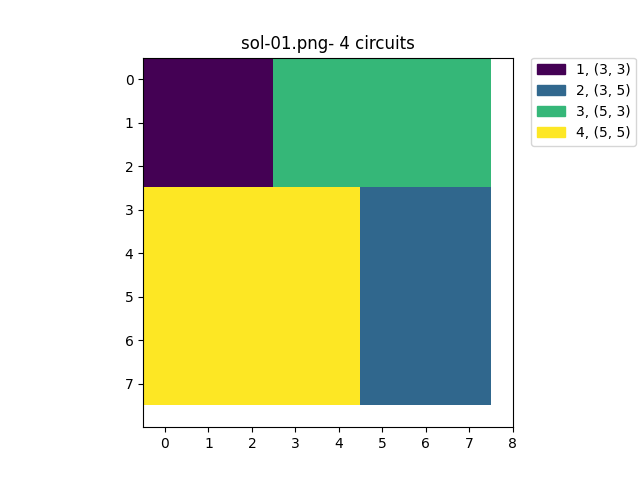
\includegraphics[width=12cm, height=10cm]{images/sol-01.png}
 \caption{Solution as image}
 \label{fig:future}
\end{figure}

\subsection{Final considerations}
By developing this project, many theoretical concepts are clarified and applied in a practical way. \\
As first step, we reasoned on how to model a problem identifying which are parameters and variables, how to encode it in different languages, such as Minizinc and SMT, then we tried to improve the model by introducing in Minizinc global constraints, implied constraints or conditions, and finally symmetry breaking constraints. We though that this procedure is much efficient. \\
Then, we did different experiments by changing configuration parameters, for Minizinc models, we found that the fastest way to find the correct solution is to apply \emph{first\_fail} as the criteria to choose the variable, and \emph{indomain\_min} to choose the value.\\

We can say that \textbf{CSP 1.3.0} seems to perform better than \textbf{SMT} and \textbf{CSP 1.0.0}, at least it should asymptotically do so. Below we have summarized some datum about the model mentioned on the \textbf{40} instances given as reference:
\begin{itemize}
    \item \textbf{Solved instances}: \textit{26};
    \item \textbf{Average solving time}: \textit{17.48s};
    \item \textbf{Total execution time for the solved instances}: \textit{454.53s}
\end{itemize}
\clearpage